\documentclass[10.5pt]{article}
\usepackage[letterpaper, margin=0.6in, top=0.5in, bottom=0.5in]{geometry}
\usepackage{amsmath,amssymb,amsthm}
\usepackage{fancyhdr}
\usepackage{xcolor}
\usepackage{tikz}
\usepackage{enumitem}
\usepackage{tcolorbox}
\usepackage{hyperref}

% Define colors matching instructor board annotations
\definecolor{chalkblue}{RGB}{0, 105, 185}
\definecolor{chalkred}{RGB}{205, 35, 35}
\definecolor{chalkpink}{RGB}{230, 90, 120}
\definecolor{chalkcyan}{RGB}{15, 160, 190}
\definecolor{chalkgreen}{RGB}{20, 130, 50}
\definecolor{boxbg}{RGB}{252, 252, 254}
\definecolor{boxframe}{RGB}{150, 160, 180}

\pagestyle{fancy}
\fancyhf{}
\renewcommand{\headrulewidth}{0pt}
\renewcommand{\footrulewidth}{0pt}

\setlength{\parindent}{0pt}
\setlength{\parskip}{2.5pt}

\begin{document}

% ==============================================================================
% PAGE 1
% ==============================================================================
\noindent \textbf{\large Math 105L} \hfill \textbf{\large Lab 7}\\[1pt]
{\textbf{\Large Inverse Functions \& Graphical Symmetry}}\\[-5pt]
\rule{\textwidth}{1.2pt}

\vspace{0.03in}

\textbf{\large Part I: Invertible Functions \& The Definition of an Inverse}

\begin{itemize}[leftmargin=1.2em, topsep=1pt, itemsep=2pt]
  \item \textbf{Core Definition:} Suppose $f$ is a function and there is a corresponding function $g$ such that $g(f(t)) = t$ and $f(g(t)) = t$ for every value of $t$ in their respective domains. Then $g$ is called the \textbf{inverse function} of $f$, denoted $\mathbf{f^{-1}}$:
  \begin{tcolorbox}[colback=boxbg, colframe=boxframe, boxrule=0.8pt, arc=3pt, left=8pt, right=8pt, top=4pt, bottom=4pt]
  \[
    \mathbf{f\big(f^{-1}(x)\big) = x = f^{-1}\big(f(x)\big)}
  \]
  \textit{Crucial Caution from Board:} Note that $\mathbf{f^{-1}(x) \neq \frac{1}{f(x)}}$! The exponent $-1$ denotes functional inversion, not the multiplicative reciprocal.
  \end{tcolorbox}
\end{itemize}

\vspace{0.02in}

\textbf{Mapping Diagram Exploration:}
Suppose $g$ is a function with domain $A = \{x, y, z\}$ and range $B = \{u, v, w\}$ such that $g(x) = u$, $g(y) = v$, and $g(z) = w$:

\begin{center}
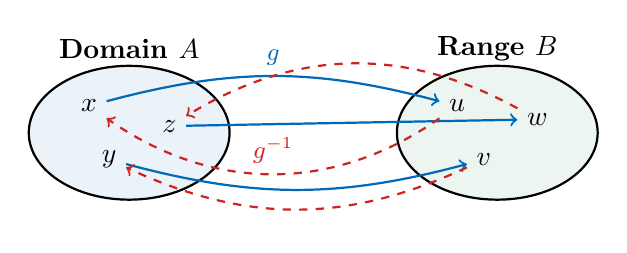
\begin{tikzpicture}[scale=0.85]
  % Set A
  \draw[thick, fill=chalkblue!8] (0,0) ellipse (1.5cm and 1cm);
  \node at (0, 1.25) {\textbf{Domain $A$}};
  \node (x) at (-0.6, 0.4) {$x$};
  \node (y) at (-0.3, -0.4) {$y$};
  \node (z) at (0.6, 0.1) {$z$};

  % Set B
  \draw[thick, fill=chalkgreen!8] (5.5,0) ellipse (1.5cm and 1cm);
  \node at (5.5, 1.25) {\textbf{Range $B$}};
  \node (u) at (4.9, 0.4) {$u$};
  \node (v) at (5.3, -0.4) {$v$};
  \node (w) at (6.1, 0.2) {$w$};

  % Forward arrows (g)
  \draw[->, thick, chalkblue] (x) to[bend left=15] node[above] {\small $g$} (u);
  \draw[->, thick, chalkblue] (y) to[bend right=15] (v);
  \draw[->, thick, chalkblue] (z) to (w);

  % Inverse arrows (g^-1)
  \draw[->, dashed, thick, chalkred] (u) to[bend left=35] node[above] {\small $g^{-1}$} (x);
  \draw[->, dashed, thick, chalkred] (v) to[bend left=25] (y);
  \draw[->, dashed, thick, chalkred] (w) to[bend right=30] (z);
\end{tikzpicture}
\end{center}

\begin{itemize}[leftmargin=1.2em, topsep=1pt, itemsep=2pt]
  \item \textbf{Describing $g^{-1}$:} Since $g^{-1}(g(t)) = t$, we must have:
  \[
    g^{-1}(u) = x, \qquad g^{-1}(v) = y, \qquad g^{-1}(w) = z
  \]
  \item \textbf{Domain and Range Swap:}
  \[
    \text{Domain}\big(g^{-1}\big) = \text{Range}(g) = \{u, v, w\}, \qquad \text{Range}\big(g^{-1}\big) = \text{Domain}(g) = \{x, y, z\}
  \]
  \item \textbf{Is $g^{-1}$ a function?} Yes, because each input in $\{u, v, w\}$ points to exactly one output in $\{x, y, z\}$.
\end{itemize}

\newpage

% ==============================================================================
% PAGE 2
% ==============================================================================
\noindent \textbf{\large Math 105L} \hfill \textbf{\large Lab 7 (Page 2)}\\[1pt]
{\textbf{\Large GeoGebra Exploration: Reflection Across $y = x$ \& Strict Monotonicity}}\\[-5pt]
\rule{\textwidth}{1.2pt}

\vspace{0.03in}

\textbf{\large GeoGebra Investigation: Symmetry across the Line $y = x$}

In the computer laboratory demonstration, we graph linear and non-linear inverse pairs:

\begin{minipage}[c]{0.52\textwidth}
  \textbf{Linear Pair Examined:}
  \begin{itemize}[leftmargin=1.2em, label=$\bullet$, topsep=1pt, itemsep=2pt]
    \item $f(x) = 2x + 3$
    \item Solve for $x$: $y = 2x + 3 \implies 2x = y - 3 \implies x = \frac{1}{2}y - \frac{3}{2}$
    \item Inverse function: $\mathbf{g(x) = f^{-1}(x) = 0.5x - 1.5}$
    \item Line of symmetry: $\mathbf{h(x) = x}$ (red dashed diagonal).
    \item \textbf{Intersection Point:} The graphs of $f(x)$ and $f^{-1}(x)$ intersect on the line $y = x$ at:
    \[
      2x + 3 = x \implies x = -3 \implies \mathbf{(-3, -3)}
    \]
  \end{itemize}
\end{minipage}%
\hfill
\begin{minipage}[c]{0.45\textwidth}
  \centering
  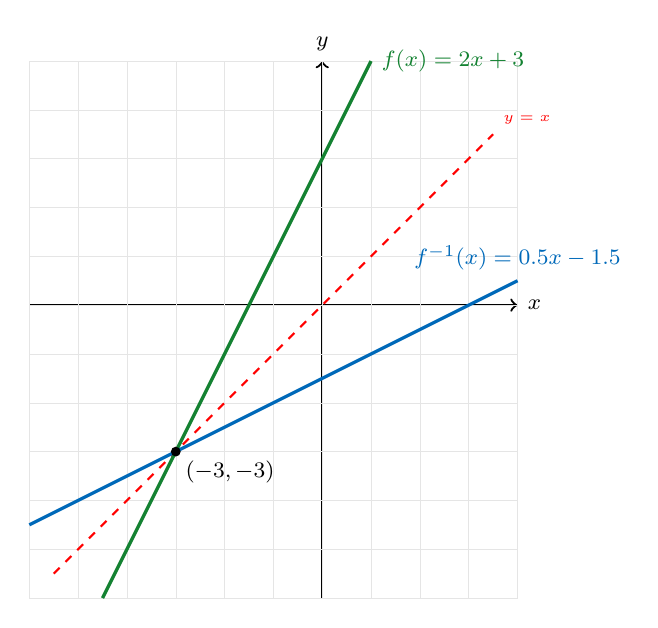
\begin{tikzpicture}[scale=0.62]
    \draw[->, thick] (-6,0) -- (4,0) node[right] {\footnotesize $x$};
    \draw[->, thick] (0,-6) -- (0,5) node[above] {\footnotesize $y$};
    \draw[step=1cm, gray!20, very thin] (-6,-6) grid (4,5);
    % Line y = x
    \draw[red, dashed, thick] (-5.5,-5.5) -- (3.5,3.5) node[above right] {\tiny $y=x$};
    % f(x) = 2x + 3
    \draw[chalkgreen, very thick] (-4.5,-6) -- (1,5) node[right] {\footnotesize $f(x) = 2x+3$};
    % g(x) = 0.5x - 1.5
    \draw[chalkblue, very thick] (-6,-4.5) -- (4,0.5) node[above] {\footnotesize $f^{-1}(x) = 0.5x - 1.5$};
    % Intersection point
    \filldraw[black] (-3,-3) circle (2.5pt) node[below right] {\footnotesize $(-3,-3)$};
  \end{tikzpicture}
\end{minipage}

\vspace{0.04in}

\textbf{\large Invertibility Without an Explicit Radical Formula: $f(x) = x^5 + x$}

Can a function be invertible even if we cannot algebraically isolate $x$?
\begin{itemize}[leftmargin=1.2em, topsep=1pt, itemsep=2pt]
  \item Consider the polynomial $f(x) = x^5 + x$.
  \item By the Abel-Ruffini theorem, there is no general formula in radicals to solve $x^5 + x = y$ for $x$.
  \item \textbf{Calculus Verification of Invertibility:}
  \[
    f'(x) = 5x^4 + 1
  \]
  Since $x^4 \ge 0$ for all real numbers $x$, we have $5x^4 \ge 0$, which guarantees:
  \[
    \mathbf{f'(x) \ge 1 > 0 \quad \text{for all } x \in (-\infty, \infty)}
  \]
  \item Because the derivative is strictly positive everywhere, $f(x)$ is \textbf{strictly increasing} across its entire domain $(-\infty, \infty)$.
  \item Any strictly increasing function \textbf{must pass the Horizontal Line Test (HLT)}.
  \item \textbf{Conclusion:} The inverse function $f^{-1}(x)$ exists, is strictly increasing, and is continuous and differentiable everywhere, even without an elementary algebraic expression!
\end{itemize}

\begin{tcolorbox}[colback=chalkblue!6, colframe=chalkblue, boxrule=1pt, arc=3pt, left=8pt, right=8pt, top=4pt, bottom=4pt]
\textbf{The Derivative Connection to Invertibility (Preparation for IFT):}\\[1pt]
If $f'(x) > 0$ everywhere (or $f'(x) < 0$ everywhere) on an interval, then $f(x)$ is strictly monotonic, passes the horizontal line test, and is guaranteed to be invertible on that interval.
\end{tcolorbox}

\end{document}

